\documentclass{jsarticle}
\usepackage{amsmath, smssymb, amsfonts}
\usepackage{newtxtext, newtxmath}
\usepackage{latexsym}
\usepackage{mathrsfs}
\usepackage{mathtools}
\usepackage[dvipdfmx]{graphicx, xcolor}
\usepackage{float}
\usepackage{wrapfig}	% must be after float package.
\usepackage{subcaption}
\usepackage{booktabs}
\usepackage{url}
\usepackage{listings, jvlisting, color}

\definecolor{OliveGreen}{rgb}{0.0,0.6,0.0}
\definecolor{Orenge}{rgb}{0.89,0.55,0}
\definecolor{SkyBlue}{rgb}{0.28, 0.28, 0.95}
\lstset{
  language={C++}, % 言語の指定
  basicstyle={\ttfamily},
  identifierstyle={\small},
  commentstyle={\smallitshape},
  keywordstyle={\small\bfseries},
  ndkeywordstyle={\small},
  stringstyle={\small\ttfamily},
  frame={tb},
  breaklines=true,
  columns=[l]{fullflexible},
  numbers=left,
  xrightmargin=0zw,
  xleftmargin=3zw,
  numberstyle={\scriptsize},
  stepnumber=1,
  numbersep=1zw,
  lineskip=-0.5ex,
  keywordstyle={\color{SkyBlue}},     %キーワード(int, ifなど)の書体指定
  commentstyle={\color{OliveGreen}},  %注釈の書体
  stringstyle=\color{Orenge}          %文字列
}


\begin{document}

\title{ゼミ レポート 04}
\author{山田朔也}
\maketitle

\section{本レポートについて}
5月24日に行われたゼミにて出題された課題に対するレポートとなっている。
課題の内容はllg方程式から、垂直磁気異方性を持つ磁性体内での1次元Bloch磁壁(以下単にBloch磁壁)の磁化構造を求めることだ。

\section{原理}
\subsection{1次元Bloch磁壁}
磁壁とは、磁気モーメントの向きが真反対を向いている磁区間にある、磁気モーメントが徐々に逆になっていく区間を指す。
また、1次元Bloch磁壁の磁化構造はx座標にのみ依存し、yおよびz方向に対しては同じ構造が無限遠方まで続いていると考える。

\subsection{静磁界}
Bloch磁壁の特徴から、
磁気モーメントに加わる静磁界は式\ref{00}で表される。
\begin{equation}
	\vec{H}^D (x) = 
	\begin{pmatrix}
		-4\pi Mx(x)\\
		0\\
		0
	\end{pmatrix}
	\label{00}
\end{equation}


\subsection{交換磁界}
磁壁にある原子磁気モーメントには、原子磁気モーメント間の角度が平行の場合に最小となるエネルギーである、交換エネルギーが働く。
以下の式\ref{01}がその交換エネルギーを表す式となる。
\begin{equation}
	\label{01}
	\varepsilon^A = A(\nabla \vec{m})^2
\end{equation}
ただし、$A$は交換スティフネス定数とする。

これを変分することで、実効磁界として扱うことができる。(式\ref{02})
\begin{equation}
	\label{02}
	\vec{H}^A = -\frac{\delta \varepsilon^A}{\delta \vec{M}}
\end{equation}

今回の問題では、1次元の磁化構造を考えるため、膜圧が無限大の構造となる。
よって、計算領域を厚さdxの区間へと分割し、それがx方向に積み重なっていると考える。
このような離散化をすると、交換磁界は
\begin{equation}
	\label{03}
	\vec{H}^A = \frac{2A}{M \delta x^2}
	\begin{pmatrix}
		m_{x_{i+1}} - 2m_{x_i} + m_{x_{i-1}}\\
		m_{y_{i+1}} - 2m_{y_i} + m_{y_{i-1}}\\
		m_{z_{i+1}} - 2m_{z_i} + m_{z_{i-1}}
	\end{pmatrix} 
\end{equation}
と表される。

\subsection{磁化構造}
静止時のBloch磁壁の磁化構造について考える。
このときの磁壁内部のエネルギーは、交換エネルギーと異方性エネルギーだけとなるため、
磁化構造はこれらのエネルギーの和が最小になる状態として考えられる。
\begin{equation}
	\int_{-\infty}^{\infty} [A(\nabla\vec{m})^2 + K_u(1-mz^2)] \,dx \rightarrow \min
\end{equation}

さらに、磁気モーメントを極座標で表したとき、磁化構造は以下の式\ref{04}, \ref{05}で表される。
\begin{equation}
	\label{04}
	\varphi(x) = \mathrm{const}(=\pm \frac{\pi}{2})
\end{equation}
\begin{equation}
	\label{05}
	\theta(x) = 2\tan ^{-1} (\exp\frac{\pi x}{l_w})
\end{equation}
ここで、$l_w$は磁壁の厚さを表す定数となり、$l_w=\pi\sqrt{A/K_u}$となる。

\section{問題}
問題内容は4次のルンゲクッタ法を用いてLLG方程式を解くプログラムを作成し、1次元Bloch磁壁の磁化構造を求めることとなる。
なお、材料定数および、各種初期値は以下のようになる。
\begin{itemize}
 \item 原子磁気モーメントの大きさ$M = 14\;\mathrm{emu/cm^3}$
 \item 交換スティフネス定数$A = 0.1\times 10^{-6}\;\mathrm{erg/cm}$
 \item 異方性定数$K_u = 10000\;\mathrm{erg/cm^3}$
 \item 損失定数$\alpha = 0.14$
 \item 磁気回転比$\lvert\gamma\rvert = 1.76\times 10^7\;\mathrm{rad/(s\cdot Oe)}$
 \item 時間刻み$\mathrm{dt} = 0.1\times 10^{-12}\;\mathrm{s}$
 \item 格子間隔を決定づける変数$\mathrm{interval} = 10$
 \item 計算点数は偶数個。
 \item 磁化構造の初期値は解析解を使用する。
\end{itemize}
ただし、実際に計算に用いる格子間隔dxの値は、磁壁幅$l_w$の$1/\mathrm{interval}$の値となる。

上記の条件下で、以下のことを計算及び調べる。
\begin{enumerate}
 \item 得られた磁化構造から磁壁の幅を調べる。
 \item 格子間隔を変化させて、求めた磁壁の幅と解析解で与えられる磁壁幅とを比較する。
 \item 格子間隔および時間幅を変化させて、計算の安定性を調べる。
\end{enumerate}
上記の項目をそれぞれ小問1-3として、以下で回答する。

\subsection{プログラム}
プログラムのアルゴリズムは以下のような流れとなった。
\begin{enumerate}
 \item 材料定数の読み込み
 \item 初期状態の計算
 \item 以下を収束するまで、時間刻みを一つ分増やしつつ繰り返し
 \begin{enumerate}
  \item 現在の磁界を、現在の磁気モーメントから算出。その後$k1$を計算する。
  \item $k1$の値を現在の磁気モーメントに反映。
  \item 現在の磁界を、現在の磁気モーメントから算出。その後$k2$を計算する。
  \item $k2$の値を現在の磁気モーメントに反映。
  \item 現在の磁界を、現在の磁気モーメントから算出。その後$k3$を計算する。
  \item $k3$の値を現在の磁気モーメントに反映。
  \item 現在の磁界を、現在の磁気モーメントから算出。その後$k4$を計算する。
  \item $k1,k2,k3,k4$の値を現在の磁気モーメントに反映。
  \item 収束判定。収束していれば繰り返しを中止。
 \end{enumerate}
\end{enumerate}

ここでの収束判定の方法だが、これは磁気モーメントに加わるトルクの平均値から求めている。
収束判定を行った時点のトルクの平均値と直前のトルクの平均値の差が、
計算開始時点のトルクの平均値との差と比べ、$1/10^{12}$以下になった時点で収束と判定している。

\subsection{小問1}
プログラムを実行したところ、解析解から少し磁気モーメントの向きが変わって収束した。
その時の様子は以下の図\ref{fig01}の様になった。
\begin{figure}[H]
	\centering
	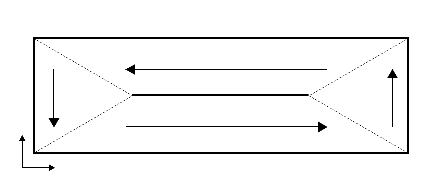
\includegraphics[width=14cm]{pic01.eps}
	\caption{Bloch磁壁の磁化構造}
	\label{fig01}
\end{figure}

また、材料定数から得られる解析解での磁壁の厚さは$l_{w_{init}} = 9.934588\times 10^{-6}\;\mathrm{cm}$だったが、
シミュレーションで得られた磁壁の厚さは$l_{w_{sim}} = 9.661578\times 10^{-6}\;\mathrm{cm}$となった。

このことから、シミュレーションでの値は解析解から得られる値と少し離れることが分かる。

\subsection{小問2}
次に格子間隔を変化させて、求めた磁壁の幅と解析解で与えられる磁壁幅とを比較する。
格子間隔dxは、intervalの値を8から2ずつ増やしていくことで変化させていく。
まず以下に、横軸が格子間隔dxで縦軸が磁壁幅$l_w$のグラフを記載する。
\begin{figure}[H]
	\centering
	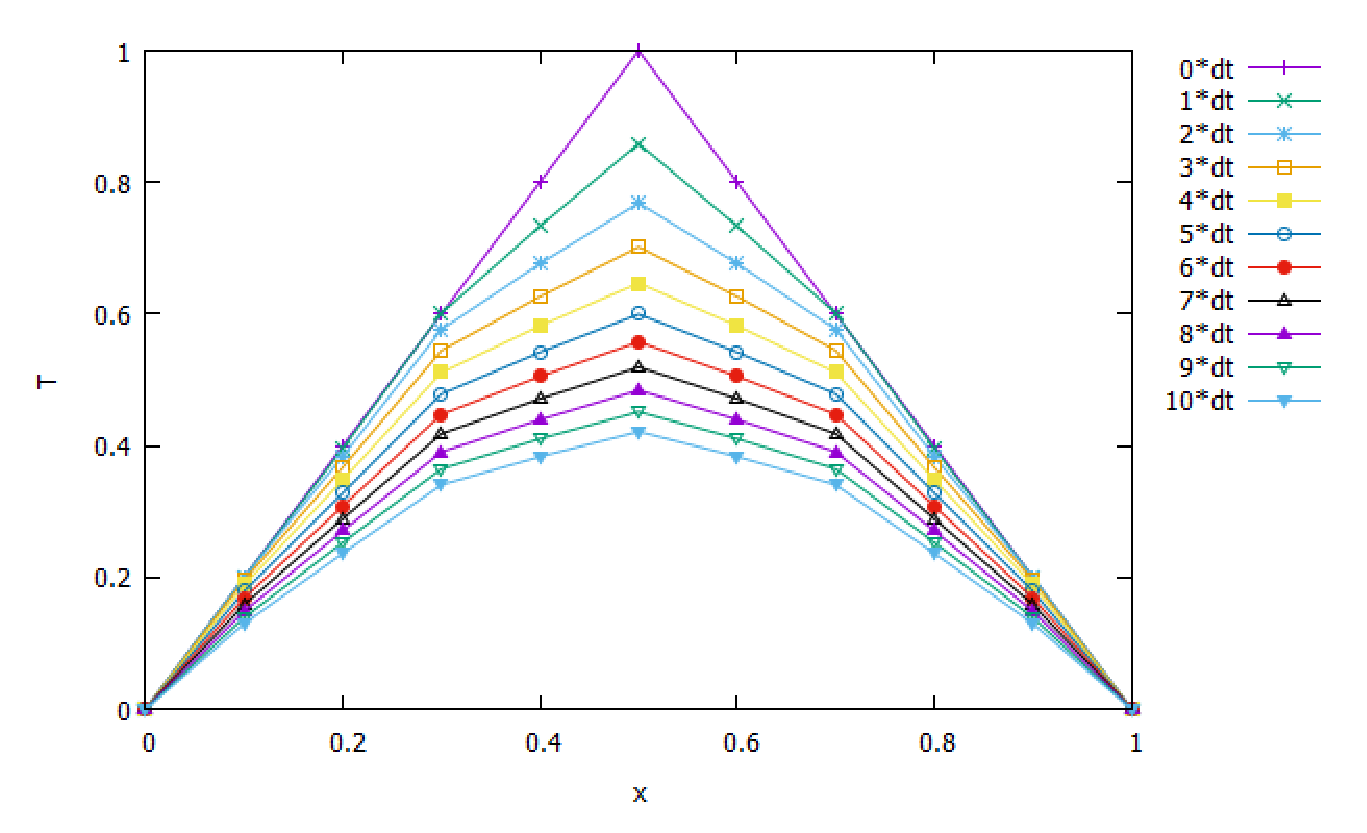
\includegraphics[width=14cm]{pic02.eps}
	\caption{磁壁幅と格子間隔の関係}
	\label{fig02}
\end{figure}

このように格子間隔を小さくすればするほど、シミュレーションで得た磁壁幅は
解析解で得た磁壁幅の値に近づいていく。

ただし、このグラフには描画していないが、このグラフに描画されている以上に格子間隔を狭めた場合、
計算が破綻してしまった。
なお、今回のシミュレーションで収束した格子間隔の最小値は$1.83974\;\mathrm{nm}$(interval$=54$)であった。

\subsection{小問3}
格子間隔及び時間幅dtを変化させて、計算の安定性を調べる。
まず、格子間隔を初期値の値に設定して、時間幅を1/10ずつ小さくしていった。
初期値の1/1000まで小さくしても、繰り返し回数は増えたものの、計算が破綻することもなく、正しく収束した。

次に時間幅dtを増やしていくと計算が破綻したため、以下のように条件を変えつつ計算が破綻しない最大のdtの値を探した。
\begin{itemize}
 \item intervalを6から54まで、4ずつ増やしていく。
 \item dtを$0.1\times 10^{-12}\;\mathrm{s}$から$0.1\times 10^{-12}$ずつ増やしていく。
\end{itemize}
この条件下で計算が破綻しない最大のdtは以下のようになった。
\begin{figure}[H]
	\centering
	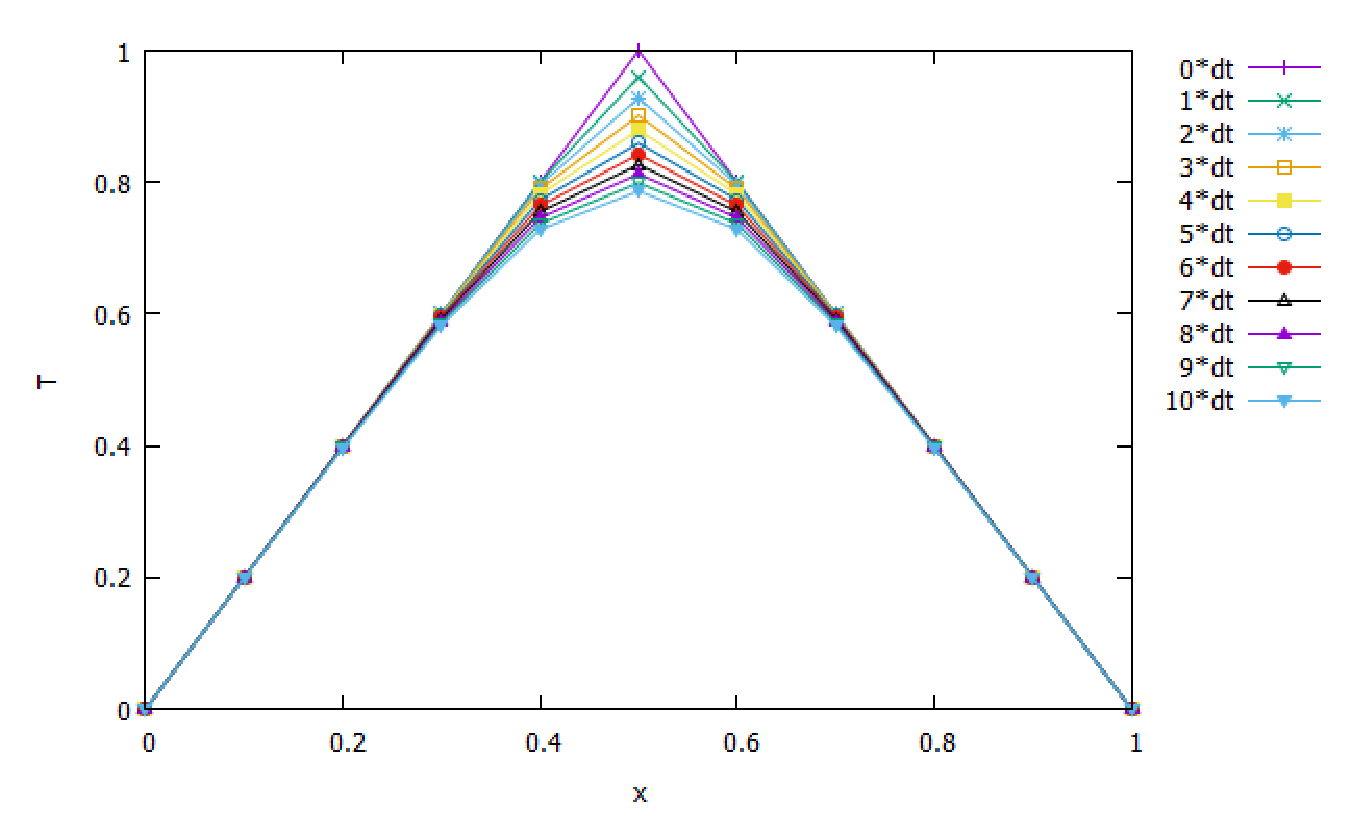
\includegraphics[width=14cm]{pic03.eps}
	\caption{格子間隔と計算が破綻しない最大のdtの関係}
	\label{fig03}
\end{figure}

この図から、格子間隔を大きくすればするほど、時間幅を大きくしても計算が破綻しない。
また、格子間隔を狭めた場合は時間幅も相応に小さくしなければ計算が破綻する、ということが分かる。

このことと、小問2から、より解析解に近い計算結果を得たければ、時間幅と格子間隔の両方を小さくしなければならない。

\section{参考文献}

\begin{itemize}
  \item 配布されたテキスト
\end{itemize}

\end{document}